

\documentclass[10pt]{beamer}

\mode<presentation>
{
 \usetheme{Boadilla}
\pagestyle{empty}

\setbeamerfont*{frametitle}{size=\normalsize,series=\bfseries}
\setbeamerfont*{block}{size=\normalsize,series=\bfseries}
%\setbeamertemplate{blocks}[rounded][shadow=true]
}

\definecolor{links}{HTML}{2A1B81}
\hypersetup{colorlinks,linkcolor=,urlcolor=links}


\usepackage[pdf]{pstricks}
\usepackage{pst-sigsys}


\definecolor{darkblue}{rgb}{0.0, 0.0, 0.40}
\setbeamercolor{title}{fg=darkblue}
\setbeamercolor{frametitle}{fg=darkblue}
\definecolor{darkgreen}{rgb}{0.0, 0.4, 0.0}

\usepackage{bbm}


\def\nn{\nonumber}
\def\xt{x(t)}
\def\xn{x[n]}
\def\xeven{x_{\text{even}}}
\def\xodd{x_{\text{odd}}}

\newcommand{\fs}[2]{#2}

\title[]{Unit Step, Impulse}
\author[\textcolor{blue}{Systems and Circuits}]{\textcolor{darkblue}{Pablo M. Olmos} (olmos@tsc.uc3m.es)\\ \textcolor{darkblue}{Emilio Parrado} (emipar@tsc.uc3m.es)}
\institute{\textcolor{white}{UC3M}}


\AtBeginSection[]
{
  \begin{frame}<beamer>{Index}
    \tableofcontents[currentsection,currentsubsection]
  \end{frame}
}






%%%%%%%%%%%%%%%%
\begin{document}

\frame{
\titlepage
\thispagestyle{empty}
\begin{center}

\includegraphics[scale=0.05]{Figures/uc3m-logo2.pdf}
\end{center}
}

\section{Discrete Unit step and Impulse}


\frame{
\begin{exampleblock}{Today}
We describe a set of  basic signal models whose properties are extremely important to analyze and design complex signal processing systems.
\end{exampleblock}

\begin{figure}
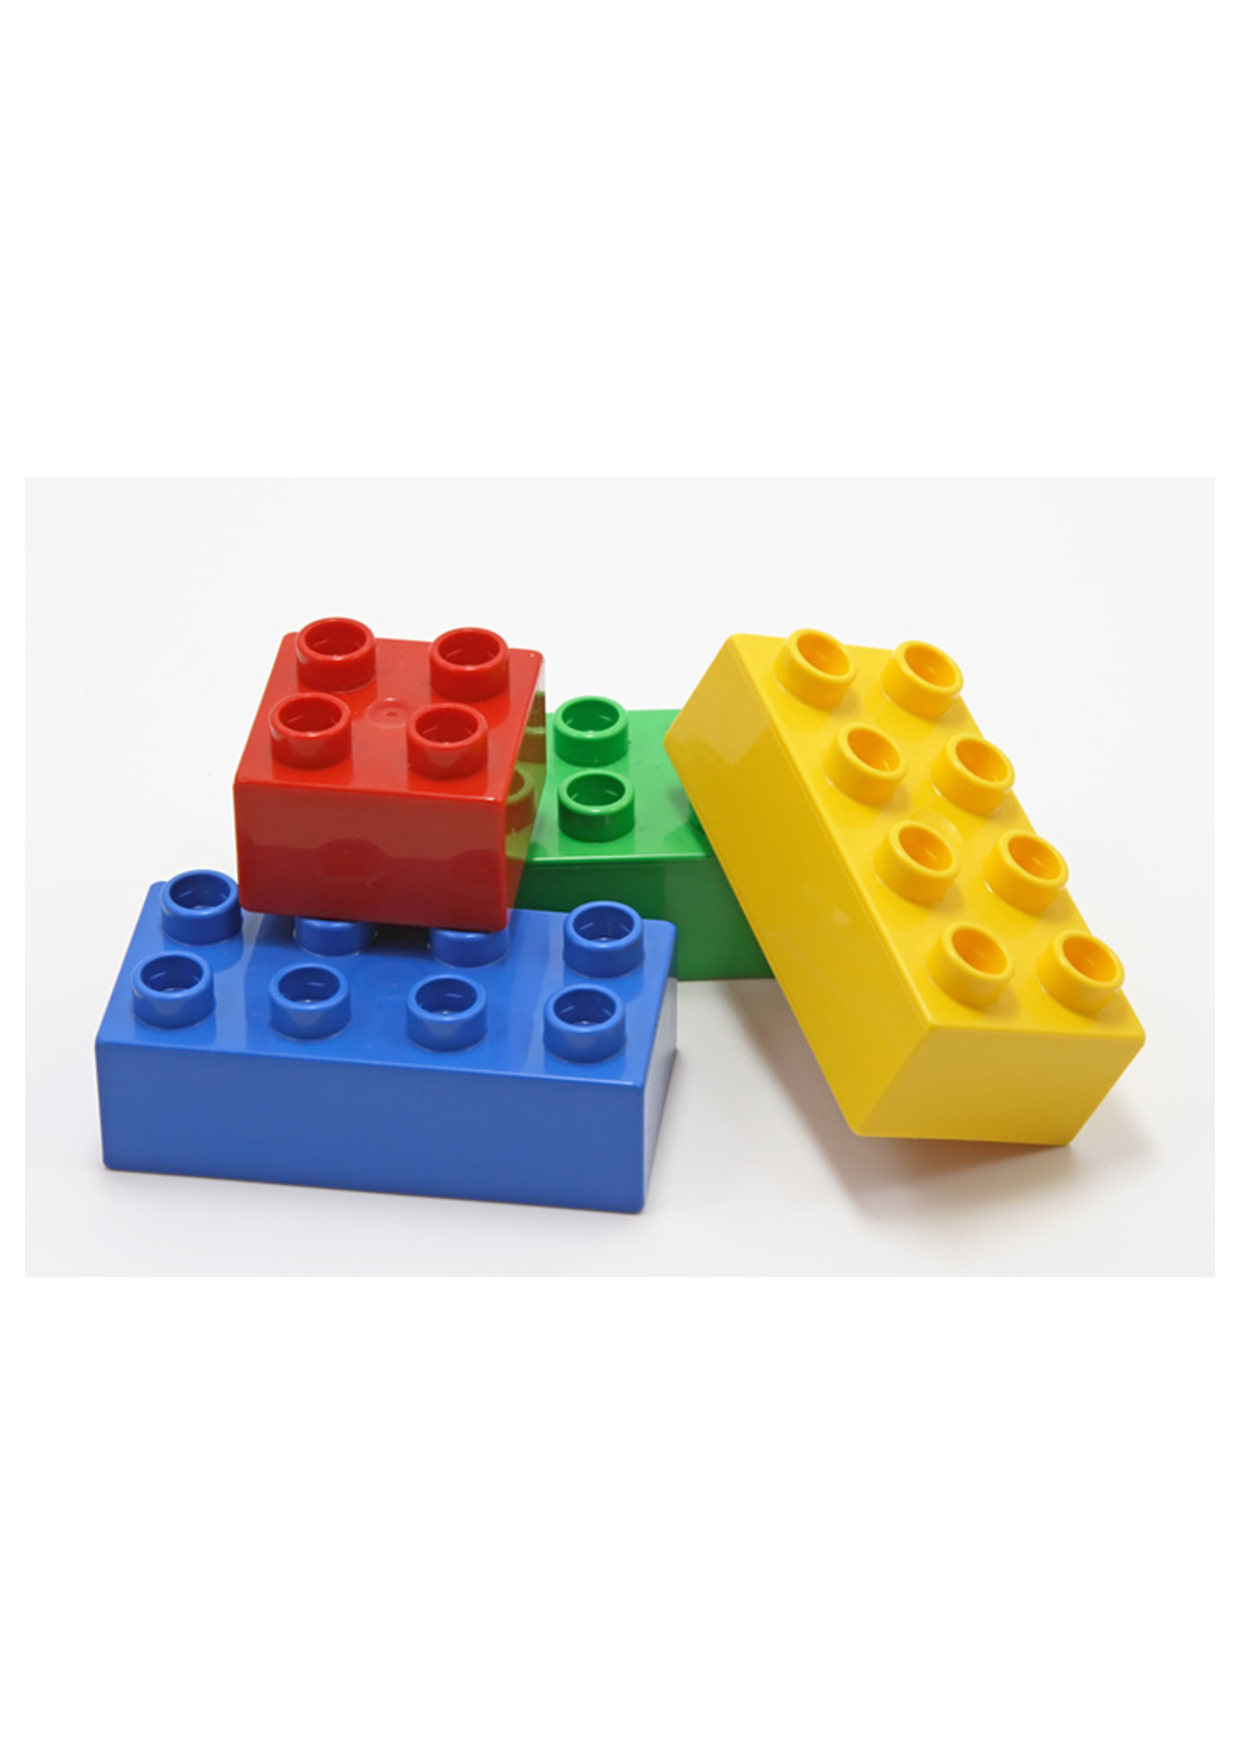
\includegraphics[scale=0.2]{Figures/Signal70.pdf}
\end{figure}

}


\frame{
\frametitle{Unit Impulse Sequence (Kronecker delta)}

Probably the simplest sequence we can imagine:
\begin{align}\nn
\delta[n]=\left\{
\begin{array}{cc}
1 & n=0\\
0 & n\neq 0
\end{array}
\right.
\qquad
\delta[n-n_0]=\left\{
\begin{array}{cc}
1 & n=n_0\\
0 & n\neq n_0
\end{array}
\right.
\end{align}


\begin{figure}
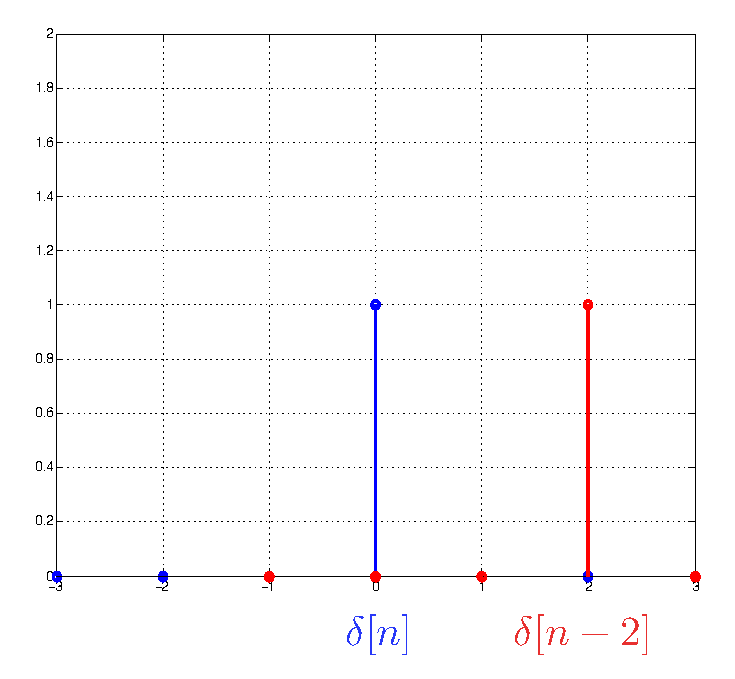
\includegraphics[scale=0.45]{Figures/Signal62.pdf}
\end{figure}

}

\frame{
\frametitle{Unit Impulse Sequence. Properties}
\begin{block}{}
It is an even signal: $\delta[n]=\delta[-n]$.
\end{block}
\begin{alertblock}{}
 Is $\delta[n-n_0]$ an even signal?
\end{alertblock}
\begin{exampleblock}{}
\begin{align}\nn
x[n]\delta[n-n_0]=\left\{
\begin{array}{cc}
x[n_0] & n=n_0\\
0 & n\neq n_0
\end{array}
\right.
\end{align}
\end{exampleblock}

\begin{block}{}
\begin{align}\nn
\sum_{n=-\infty}^{\infty}\delta[n]=1
\end{align}
\end{block}

\begin{exampleblock}{}
$\delta[n]$ is a signal of finite energy.
\end{exampleblock}

}

\frame{
\frametitle{Unit Impulse Sequence. Properties}

\begin{block}{}
Any signal can be decomposed as a sum of unit impulse sequences:
\begin{align}\nn
x[n]=\sum_{k=-\infty}^{\infty}x[k]\delta[n-k]
\end{align}
\end{block}

\begin{figure}
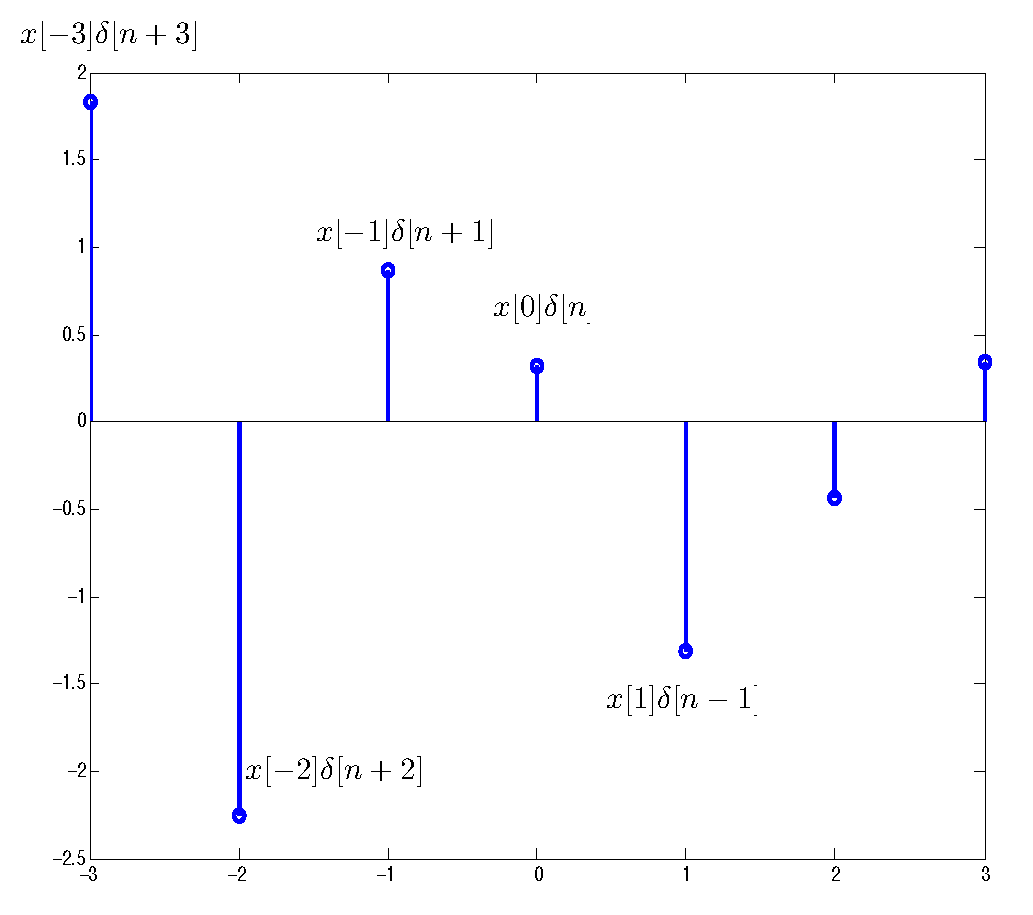
\includegraphics[scale=0.35]{Figures/Signal64.pdf}
\end{figure}
}

\frame{
\frametitle{Unit Step Sequence}

 \begin{align}\nn
u[n]=\left\{
\begin{array}{cc}
1 & n\geq0\\
0 & n< 0
\end{array}
\right.
\end{align}

\begin{block}{From $\delta[n]$ to $u[n]$}
As we have seen, we can decompose it as a sum of unit impulse sequences:
\begin{align}\nn
u[n]&=\sum_{k=-\infty}^{\infty}u[k]\delta[n-k]=\sum_{0}^{\infty}\delta[n-k]\\\nn
u[n-n_0]&=\sum_{k=-\infty}^{\infty}u[k-n_0]\delta[n-k]=\sum_{n_0}^{\infty}\delta[n-k]
\end{align}
\end{block}
}

\frame{
\frametitle{Unit Step Sequence}

\begin{block}{From $u[n]$ to $\delta[n]$}

We can also obtain $\delta[n]$ from $u[n]$:

\begin{align}\nn
\delta[n]&=u[n]-u[n-1]\\\nn
\delta[n-n_0]&=u[n-n_0]-u[n-n_0-1]
\end{align}
\end{block}


}

\section{Continuous-time Unit Step and Unit Impulse}

\frame{
\frametitle{Unit Step signal}
Similar to the discrete case:
\begin{align}
\nn
u(t)=\left\{
\begin{array}{cc}
1 & t\geq0\\
0 & t< 0
\end{array}
\right.
\end{align}

\begin{block}{Continuous approximation}
Let 
\begin{align}
\nn
u_L(t)=\left\{
\begin{array}{cc}
0 & t<0\\
t/L & 0<t<L\\
1 & t\geq L
\end{array}
\right.
\end{align}
then
\begin{align}\nn
\lim_{L\rightarrow 0}u_L(t)=u(t)
\end{align}
\end{block}


}


%\frame{
%\frametitle{Rectangular pulse}
%
%\begin{align}
%\nn
%\Pi(t)=\left\{
%\begin{array}{cc}
%1 & |t|\leq\frac{1}{2}\\
%0 & \text{otherwise}
%\end{array}
%\right.
%\end{align}
%
%In general:
%\begin{align}
%\nn
%\Pi\left(\frac{t-a}{b}\right)=\left\{
%\begin{array}{cc}
%1 & |t-a|\leq\frac{b}{2}\\
%0 & \text{otherwise}
%\end{array}
%\right.
%\end{align}
%
%\begin{figure}
%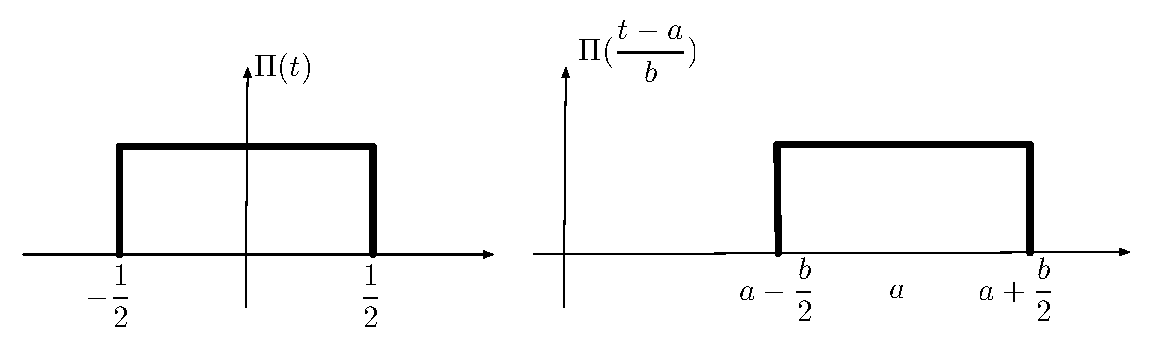
\includegraphics[scale=0.6]{Figures/Signal65.pdf}
%\end{figure}
%
%}
%
%\frame{
%\frametitle{Rectangular pulse}
%
%It can be defined in terms of the unit step signal $u(t)$:
%\begin{align}\nn
%\Pi(t)&=u(t+\frac{1}{2})-u(t-\frac{1}{2})\\\nn
%\Pi(\frac{t-a}{b})&=u(t-(a-\frac{b}{2}))-u(t-(a+\frac{b}{2}))
%\end{align}
%
%
%}

\frame{
\frametitle{Continuous-time impulse (Dirac Delta function)}

The continuous-time impulse function $\delta(t)$ is related to the unit step by the equation
\begin{align*}
u(t)=\int_{-\infty}^{t}\delta(\tau)d\tau
\end{align*}
and this suggests that
\begin{align}\nn
\delta(t)=\frac{\partial u(t)}{\partial t}=\left\{
\begin{array}{cc}
\infty & t=0\\
0 & t\neq0
\end{array}
\right.
\end{align}

\begin{figure}
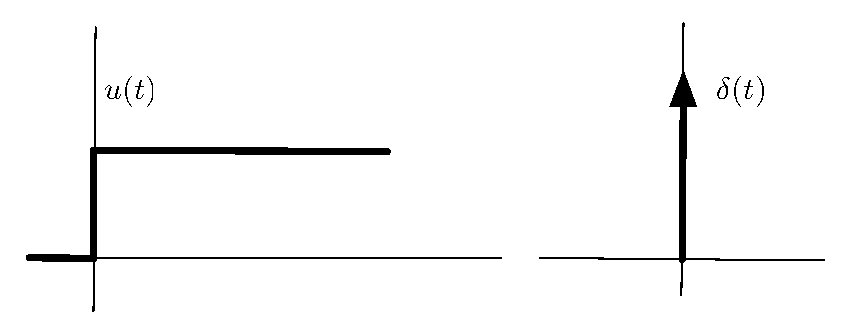
\includegraphics[scale=0.6]{Figures/Signal66.pdf}
\end{figure}

}

\frame{
\frametitle{Continuous-time impulse (Dirac Delta function)}

\begin{block}{Continuous approximation}
Let 
\begin{align}
\nn
\delta_L(t)=\frac{\partial u_L(t)}{\partial t}\left\{
\begin{array}{cc}
L^{-1} & 0<t<L\\
0 & \text{ otherwise }
\end{array}
\right.
\end{align}
then
\begin{align}\nn
\delta(t)=\lim_{L\rightarrow 0}\delta_L(t)
\end{align}
\end{block}

\begin{figure}
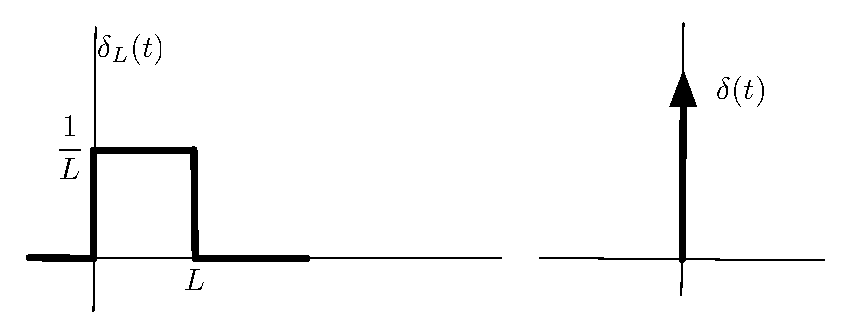
\includegraphics[scale=0.5]{Figures/Signal67.pdf}
\end{figure}

}

\frame{
For any $L$ value,
\begin{align}\nn
&\int_{-\infty}^{\infty}\delta_L(t) dt=L\frac{1}{L}=1 \Rightarrow  \int_{-\infty}^{\infty} \delta(t)=1.
\end{align}

\begin{exampleblock}{}
The signal $\delta(t)$ has unit area.
\end{exampleblock}

\begin{block}{}
\begin{align}\nn
\int_{-\infty}^{\infty}\delta(t-t_0)dt=1
\end{align}
\end{block}

}

\frame{
\frametitle{Continuous-time Impulse. Properties.}

\begin{block}{Multiplication by a constant $\rightarrow$ Area multiplication}
\begin{align}\nn
\int_{-\infty}^{\infty}k\delta(t)dt=k\int_{-\infty}^{\infty}\delta(t)dt=k
\end{align}
\end{block}

\begin{exampleblock}{$x(t)\delta(t-t_0)$}
\begin{align}\nn
x(t)\delta(t-t_0)=x(t_0)\delta(t-t_0)
\end{align}
\end{exampleblock}

\begin{figure}
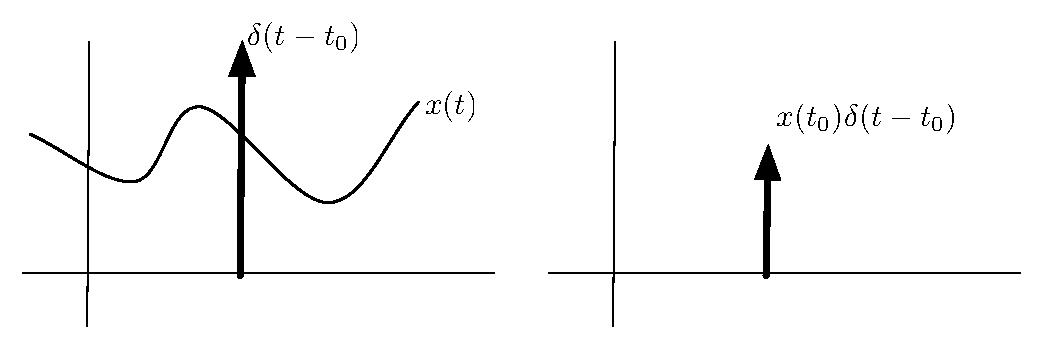
\includegraphics[scale=0.5]{Figures/Signal68.pdf}
\end{figure}

}

\frame{
\frametitle{Continuous-time Impulse. Properties (II).}

Any signal $x(t)$ can be decomposed as a linear combination of an infinite number of impulses:
\begin{align}\nn
x(t)=\int_{-\infty}^{\infty}x(\tau)\delta(t-\tau) d\tau
\end{align}

\begin{exampleblock}{Unit step signal}
\begin{align}\nn
u(t)=\int_{-\infty}^{\infty}u(\tau)\delta(t-\tau) d\tau=\int_{0}^{\infty}\delta(t-\tau) d\tau
\end{align}
\end{exampleblock}

}

\frame{
\textbf{{\color {darkblue} We approximate} $x(t)$} by a lineal combination of delayed and scaled versions of  $\delta_{L}(t)$

\begin{figure}
\centering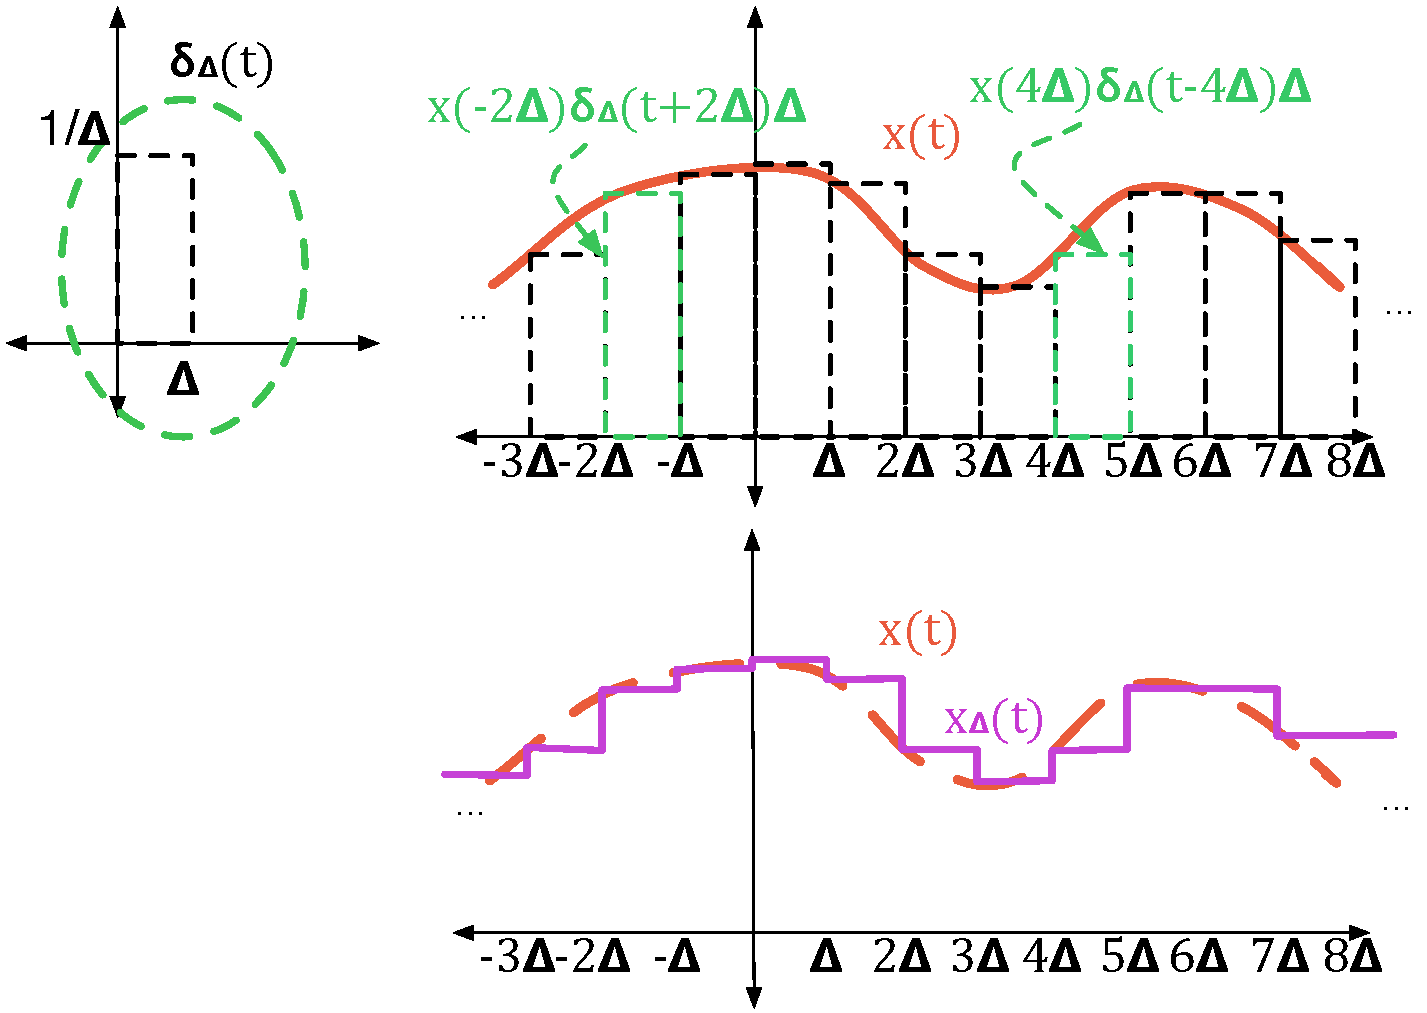
\includegraphics[scale=0.4]{Figures/Signal322.pdf}
\end{figure}
}

\frame{
\frametitle{Continuous-time Impulse. Properties (II).}
\[
x(t) \approx x_{L}(t) = \sum_{k=-\infty}^{\infty}{x(kL){\color{darkblue}\delta_{L}(t-kL)}L} 
\]

If we take the limit $L \rightarrow 0$:
\begin{itemize}
\item $kL \rightarrow \tau$
\item $\sum \rightarrow \int$
\item $L \rightarrow d\tau$
\end{itemize}

\begin{align}\nn
x(t)=\int_{-\infty}^{\infty}x(\tau)\delta(t-\tau) d\tau
\end{align}

}

\frame{
\frametitle{Relationship with the rectangular pulse}

\begin{figure}
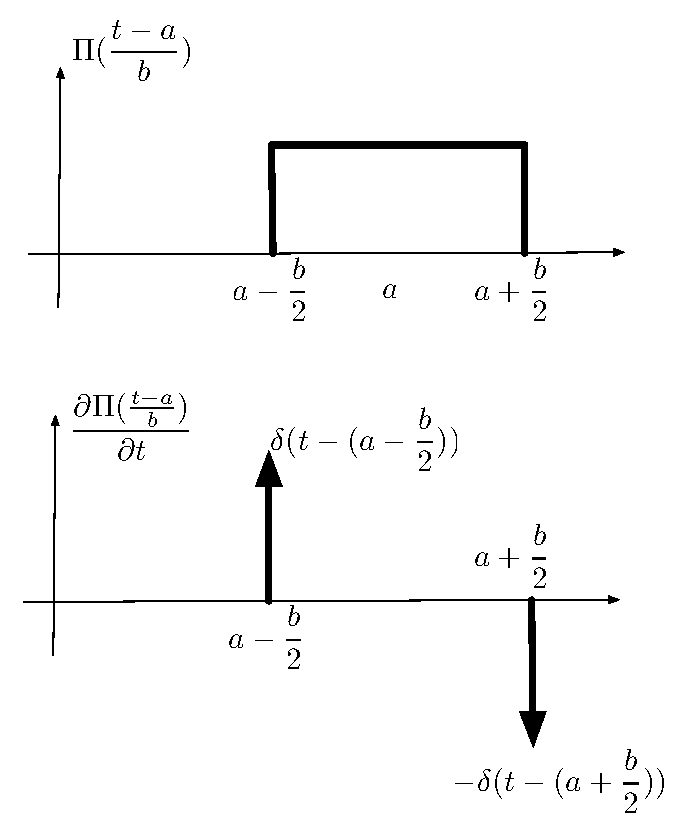
\includegraphics[scale=0.5]{Figures/Signal69.pdf}
\end{figure}

}


\end{document}
